\documentclass{article}
\usepackage[margin=1in]{geometry}
\usepackage{amsmath, amssymb, amsthm}
\usepackage{tikz}
\usetikzlibrary{arrows.meta, shapes.geometric, positioning}
\usepackage{enumitem}
\usepackage[most]{tcolorbox}
\usepackage{fancyhdr}
\usepackage{graphicx}
\usepackage[pdfborder={0 0 0}]{hyperref}
\usepackage{xcolor}
\usepackage{multicol}
\usepackage{array}
\usepackage{booktabs}
\usepackage{longtable}
\usepackage{pifont}
\usepackage{tabularx}

% =============================
% COLOR DEFINITIONS (kept consistent with companion guides)
% =============================
\definecolor{instantgreen}{RGB}{46, 204, 113}
\definecolor{minimalblue}{RGB}{52, 152, 219}
\definecolor{targetedorange}{RGB}{230, 126, 34}
\definecolor{standardpurple}{RGB}{155, 89, 182}
\definecolor{thoroughred}{RGB}{231, 76, 60}
\definecolor{multimethod}{RGB}{241, 196, 15}
\definecolor{completegray}{RGB}{149, 165, 166}
\definecolor{formalblack}{RGB}{44, 62, 80}
\definecolor{peerreview}{RGB}{22, 160, 133}
\definecolor{timingblue}{RGB}{41, 128, 185}
\definecolor{strategyGold}{RGB}{255, 215, 0}
\definecolor{trainingBlue}{RGB}{50, 215, 255}
\definecolor{contextpink}{RGB}{255, 182, 193}
\definecolor{specializedcyan}{RGB}{0, 206, 209}
\definecolor{warningred}{RGB}{192, 57, 43}
\definecolor{successgreen}{RGB}{39, 174, 96}

% =============================
% TCOLORBOX ENVIRONMENTS
% =============================

% Instant Gut Check Box (1-3 seconds)
\newtcolorbox{instantbox}[1]{
    colback=instantgreen!10,
    colframe=instantgreen!75!black,
    title={\textbf{\checkmark{} INSTANT GUT CHECK: #1}},
    fonttitle=\bfseries,
    coltitle=white,
    breakable,
    enhanced,
    attach boxed title to top left={yshift=-2mm, xshift=2mm},
    boxed title style={colback=instantgreen!75!black},
    after title={\hfill\textcolor{white}{\textbf{1-3 seconds}}}
}

% Minimal/Rapid Sanity Check Box (5-10 seconds)
\newtcolorbox{minimalbox}[1]{
    colback=minimalblue!10,
    colframe=minimalblue!75!black,
    title={\textbf{\checkmark{} MINIMAL SANITY CHECK: #1}},
    fonttitle=\bfseries,
    coltitle=white,
    breakable,
    enhanced,
    attach boxed title to top left={yshift=-2mm, xshift=2mm},
    boxed title style={colback=minimalblue!75!black},
    after title={\hfill\textcolor{white}{\textbf{5-10 seconds}}}
}

% Targeted Spot Check Box (15-30 seconds)
\newtcolorbox{targetedbox}[1]{
    colback=targetedorange!10,
    colframe=targetedorange!75!black,
    title={\textbf{\checkmark{} TARGETED SPOT CHECK: #1}},
    fonttitle=\bfseries,
    coltitle=white,
    breakable,
    enhanced,
    attach boxed title to top left={yshift=-2mm, xshift=2mm},
    boxed title style={colback=targetedorange!75!black},
    after title={\hfill\textcolor{white}{\textbf{15-30 seconds}}}
}

% Standard Verification Box (30-60 seconds)
\newtcolorbox{standardbox}[1]{
    colback=standardpurple!10,
    colframe=standardpurple!75!black,
    title={\textbf{\checkmark{} STANDARD VERIFICATION: #1}},
    fonttitle=\bfseries,
    coltitle=white,
    breakable,
    enhanced,
    attach boxed title to top left={yshift=-2mm, xshift=2mm},
    boxed title style={colback=standardpurple!75!black},
    after title={\hfill\textcolor{white}{\textbf{30-60 seconds}}}
}

% Thorough Verification Box (1-3 minutes)
\newtcolorbox{thoroughbox}[1]{
    colback=thoroughred!10,
    colframe=thoroughred!75!black,
    title={\textbf{\checkmark{} THOROUGH VERIFICATION: #1}},
    fonttitle=\bfseries,
    coltitle=white,
    breakable,
    enhanced,
    attach boxed title to top left={yshift=-2mm, xshift=2mm},
    boxed title style={colback=thoroughred!75!black},
    after title={\hfill\textcolor{white}{\textbf{1-3 minutes}}}
}

% Multi-Method Verification Box (3-5 minutes)
\newtcolorbox{multimethodbox}[1]{
    colback=multimethod!10,
    colframe=multimethod!75!black,
    title={\textbf{\checkmark{} MULTI-METHOD VERIFICATION: #1}},
    fonttitle=\bfseries,
    coltitle=black,
    breakable,
    enhanced,
    attach boxed title to top left={yshift=-2mm, xshift=2mm},
    boxed title style={colback=multimethod!75!black},
    after title={\hfill\textcolor{black}{\textbf{3-5 minutes}}}
}

% Complete Mathematical Verification Box (5-10 minutes)
\newtcolorbox{completebox}[1]{
    colback=completegray!10,
    colframe=completegray!75!black,
    title={\textbf{\checkmark{} COMPLETE VERIFICATION: #1}},
    fonttitle=\bfseries,
    coltitle=white,
    breakable,
    enhanced,
    attach boxed title to top left={yshift=-2mm, xshift=2mm},
    boxed title style={colback=completegray!75!black},
    after title={\hfill\textcolor{white}{\textbf{5-10 minutes}}}
}

% Formal Proof-Level Box (10+ minutes)
\newtcolorbox{formalbox}[1]{
    colback=formalblack!10,
    colframe=formalblack!75!black,
    title={\textbf{\checkmark{} FORMAL PROOF VERIFICATION: #1}},
    fonttitle=\bfseries,
    coltitle=white,
    breakable,
    enhanced,
    attach boxed title to top left={yshift=-2mm, xshift=2mm},
    boxed title style={colback=formalblack!75!black},
    after title={\hfill\textcolor{white}{\textbf{10+ minutes}}}
}

% Strategy Box
\newtcolorbox{strategybox}[1]{
    colback=strategyGold!10,
    colframe=strategyGold!75!black,
    title={\textbf{\checkmark{} STRATEGY: #1}},
    fonttitle=\bfseries,
    coltitle=black,
    breakable,
    enhanced,
    attach boxed title to top left={yshift=-2mm, xshift=2mm},
    boxed title style={colback=strategyGold!75!black}
}

% Training Box
\newtcolorbox{trainingbox}[1]{
    colback=trainingBlue!10,
    colframe=trainingBlue!75!black,
    title={\textbf{\checkmark{} TRAINING: #1}},
    fonttitle=\bfseries,
    coltitle=white,
    breakable,
    enhanced,
    attach boxed title to top left={yshift=-2mm, xshift=2mm},
    boxed title style={colback=trainingBlue!75!black}
}

% Context Box
\newtcolorbox{contextbox}[1]{
    colback=contextpink!20,
    colframe=contextpink!75!black,
    title={\textbf{\checkmark{} CONTEXT: #1}},
    fonttitle=\bfseries,
    coltitle=black,
    breakable,
    enhanced,
    attach boxed title to top left={yshift=-2mm, xshift=2mm},
    boxed title style={colback=contextpink!75!black}
}

% Specialized Methods Box
\newtcolorbox{specializedbox}[1]{
    colback=specializedcyan!10,
    colframe=specializedcyan!75!black,
    title={\textbf{\checkmark{} SPECIALIZED METHOD: #1}},
    fonttitle=\bfseries,
    coltitle=white,
    breakable,
    enhanced,
    attach boxed title to top left={yshift=-2mm, xshift=2mm},
    boxed title style={colback=specializedcyan!75!black}
}

% Warning Box
\newtcolorbox{warningbox}[1]{
    colback=warningred!10,
    colframe=warningred!75!black,
    title={\textbf{\textbf{!} WARNING: #1}},
    fonttitle=\bfseries,
    coltitle=white,
    breakable,
    enhanced,
    attach boxed title to top left={yshift=-2mm, xshift=2mm},
    boxed title style={colback=warningred!75!black}
}

% Success Rate Box
\newtcolorbox{successbox}[1]{
    colback=successgreen!10,
    colframe=successgreen!75!black,
    title={\textbf{\checkmark{} SUCCESS RATES: #1}},
    fonttitle=\bfseries,
    coltitle=white,
    breakable,
    enhanced,
    attach boxed title to top left={yshift=-2mm, xshift=2mm},
    boxed title style={colback=successgreen!75!black}
}

% =============================
% CUSTOM COMMANDS
% =============================
\newcommand{\timetarget}[1]{\textcolor{timingblue}{\textbf{[#1]}}}
\newcommand{\crossmark}{\ding{55}}
\newcommand{\problemrange}[1]{\textbf{Problems #1}}

% =============================
% DOCUMENT SETTINGS
% =============================
\pagestyle{fancy}
\fancyhf{}
\rhead{AMC12 \& COMC Late-Band Mastery}
\lhead{Competition Mathematics Strategy}
\cfoot{\thepage}

\title{\textbf{AMC12 \& COMC Late-Band Mastery Guide}\\
\Large Mastering AMC12 Problems 21--25 and COMC Part C\\
\large Strategy, Conversions, and Complete Verification}
\author{Advanced Competition Mathematics Series}
\date{\today}

\begin{document}

\maketitle

\begin{center}
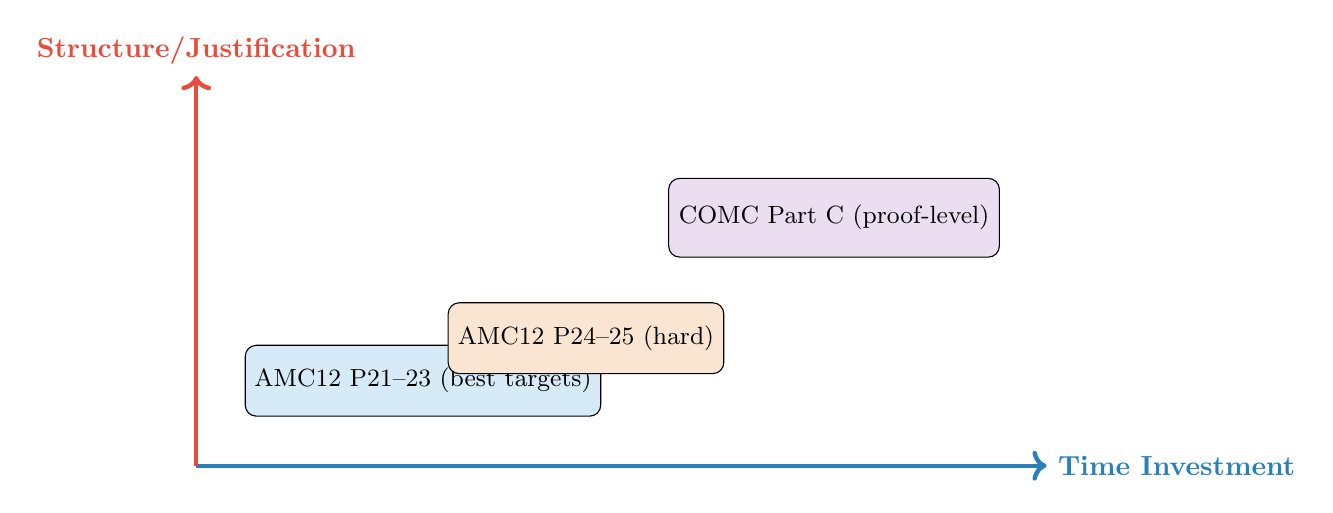
\begin{tikzpicture}[scale=0.9]
    \draw[ultra thick, ->, timingblue] (0,0) -- (12,0) node[right] {\textbf{Time Investment}};
    \draw[ultra thick, ->, thoroughred] (0,0) -- (0,5.5) node[above] {\textbf{Structure/Justification}};

    % Late-band regions
    \node[draw, rounded corners, fill=minimalblue!20, minimum width=3.5cm, minimum height=0.9cm] at (3.2,1.2) {\small AMC12 P21--23 (best targets)};
    \node[draw, rounded corners, fill=targetedorange!20, minimum width=3.5cm, minimum height=0.9cm] at (5.5,1.8) {\small AMC12 P24--25 (hard)};
    \node[draw, rounded corners, fill=standardpurple!20, minimum width=4.2cm, minimum height=1.0cm] at (9,3.5) {\small COMC Part C (proof-level)};
\end{tikzpicture}
\end{center}

\vspace{0.5em}
\noindent\textit{Companion guides:} See \emph{Early/Mid-Band Mastery} (guides/AMC12\_COMC\_Early\_Mid\_Band\_Mastery\_Guide.tex), \emph{Conversion Techniques} (guides/AMC12\_COMC\_Conversion\_Techniques.tex), and \emph{Complete Verification Methods} (guides/AMC12\_COMC\_Complete\_Verification\_Methods.tex).

\tableofcontents
\newpage

% =============================
% EXECUTIVE SUMMARY
% =============================
\section{Executive Summary}

\begin{strategybox}{Late-Band Core Principles}
\begin{itemize}[nosep]
\item \textbf{Solve by accessibility, not order}: In AMC12 late band, P20 may be easier than P18. Scan all five \timetarget{45--60s}.
\item \textbf{3-minute rule for AMC12 late-band}: If no clear traction by \timetarget{3:00}, bank the partial insight and switch.
\item \textbf{Exploit MC structure}: Bound, eliminate, and reverse-engineer from answer forms when possible.
\item \textbf{Make it easier}: Normalize, reparameterize, or analyze a nearby simpler problem, then transfer.
\item \textbf{Proof-first mindset for COMC C}: Write to convince. State targets, justify every claim, and plan for partial credit.
\item \textbf{Verification matches stakes}: Use \emph{Standard/Thorough} for AMC late band; \emph{Complete/Formal} elements for COMC C.
\end{itemize}
\end{strategybox}

\begin{contextbox}{Where This Guide Fits}
This guide focuses on late-band execution for AMC12 (P21--25) and COMC Part C. For tactical conversions (invariants, extremal, coordinate/complex, generating functions, modular arithmetic), use the companion \emph{Conversion Techniques}. For high-confidence closing, use \emph{Complete Verification Methods}.
\end{contextbox}

\newpage

% =============================
% DECODING LATE-BAND DIFFICULTY
% =============================
\section{Decoding Late-Band Difficulty}

\textit{Having established the core principles, we now examine the cognitive and structural factors that make late-band problems uniquely challenging---understanding these mechanisms is essential for developing effective solution strategies.}

\begin{contextbox}{Cognitive and Format Drivers}
Drawing on \emph{Decoding competition math difficulty}, late-band problems deliberately exceed working-memory limits and disguise familiar structures:
\begin{itemize}
    \item \textbf{Cognitive load}: 6--8 interacting constraints exceed the 2--4 chunk working memory limit, creating \emph{intrinsic cognitive load} that forces structure-first thinking.
    \item \textbf{Surface vs. deep structure}: Problems force cognitively demanding System 2 (analytical) processing rather than automatic System 1 (pattern recognition), hiding standard tactics behind novel contexts.
    \item \textbf{Format pressure}: AMC12 multiple-choice enables elimination but punishes over-solving; COMC C requires written proof-quality justification with partial credit opportunities.
\end{itemize}
\end{contextbox}

\begin{strategybox}{Operational Framework}
Use an OODA-style loop under time: \textbf{Observe} (scan), \textbf{Orient} (identify structure: algebra/NT/comb/geo), \textbf{Decide} (pick the least-cost conversion), \textbf{Act} (execute with targeted verification). Avoid anchoring; pivot after fixed time budgets.
\end{strategybox}

\begin{successbox}{Difficulty Benchmarks}
\begin{itemize}[nosep]
\item AMC12 P21--25: AoPS Level 4 (equivalent to hardest AIME 4--6, usual AIME 7--10); significant jump from P20.
\item COMC Part C: AoPS 6--10; proof-based with generous partial credit (40 points total: 4 problems × 10 points each).
\item Statistical reality: >80\% solve AMC12 P1--8; <20\% solve P21--25.
\end{itemize}
\end{successbox}

\newpage

% =============================
% AMC12 Late-Band Problems
% =============================
\section{AMC12 Late-Band Problems: Triage, Attacks, Closers}

\textit{With the difficulty framework established, we now turn to practical execution strategies for AMC12's most challenging problems---these techniques form the bridge between AMC12 mastery and AIME readiness.}

\subsection{Selection and Pacing}
\begin{strategybox}{Time and Triage}
\begin{itemize}
    \item \textbf{First pass} \timetarget{3--4 min total}: Tag the most accessible of late-band by domain comfort and visible structure cues (symmetry, factorability, small-case testability).
    \item \textbf{Per attempt} \timetarget{2:30--4:00}: Commit to a conversion and push to a resolvable subgoal. If stuck at \timetarget{3:00}, switch.
    \item \textbf{Endgame} \timetarget{5--7 min left}: Verify high-confidence solves; revisit one promising partial.
\end{itemize}
\end{strategybox}

\subsection{The Late-Band Strategy Playbook}
\textit{Combine domain-specific tactics with systems that keep your working memory clear.}
%\begin{multicols}{2}
\begin{strategybox}{Answer-Choice Leverage}
\textbf{Use when}: Bounds, parity/mod patterns, recognizable forms.\\
\textbf{How}: Bracket with monotonicity/estimates, test residues, reverse-engineer target forms (e.g., $\sqrt{a}-\sqrt{b}$, $\tfrac{p}{q}$).\\
\textbf{Outcome}: Rapid pruning; directs algebra toward the answer's template.
\end{strategybox}

\begin{strategybox}{Make It Easier}
\textbf{Use when}: Messy constants/positions; near symmetry; no traction.\\
\textbf{How}: Normalize (translate/scale/rotate), strengthen/weaken constraints, analyze toy/limit cases, then transfer pattern back and validate domain/boundaries.
\end{strategybox}

\begin{strategybox}{Penultimate Step}
\textbf{Use when}: Target form/value is clear.\\
\textbf{How}: State “It suffices to show ...”; reverse-engineer a last key relation/configuration; pick substitutions/models making the last step inevitable; ensure feasibility.
\end{strategybox}

\begin{strategybox}{Wishful Thinking}
\textbf{Use when}: Nearly factorable/closed form; likely equality case; geometric concurrency/cyclicity suspected.\\
\textbf{How}: Assume the structure with parameters, derive consequences, solve parameters, and repair rigor.
\end{strategybox}

\begin{strategybox}{Conjecture via Small Cases}
\textbf{Use when}: Opaque structure; processes/recurrences; modular patterns.\\
\textbf{How}: Compute tiny instances, record invariants/periodicity, conjecture precise form, then verify against choices or prove generally.
\end{strategybox}

\begin{center}
\begin{tabular}{|l|c|l|}
\hline
\textbf{Strategy} & \textbf{Hit Rate (heuristic)} & \textbf{Best Context} \\
\hline
Answer-Choice Leverage & 75--90\% & Numeric targets, patterned answers, estimable quantities \\
Make It Easier & 70--85\% & Geometry normalization, scale-free algebra, toy problems \\
Penultimate Step & 65--80\% & Identity targets, extremal/equality cases \\
Wishful Thinking & 60--75\% & Near-factorable algebra, concurrency/cyclicity in geometry \\
Conjecture via Small Cases & 55--70\% & Recurrences, residue cycles, combinatorial processes \\
\hline
\end{tabular}
\end{center}

\noindent\small\textit{Hit rates are heuristic guidance based on practice trends; use them to prioritize, not as guarantees.}

\subsection{Conversion Toolkit (use with companion guide)}
\begin{specializedbox}{High-Yield Conversions for late-band}
\begin{itemize}
    \item \textbf{Algebra}: Vieta/Vieta jumping; Simon's Favorite Factoring Trick; completing the square; rational parametrization; functional equations (patterns and substitutions); bounding with AM--GM/Cauchy--Schwarz.
    \item \textbf{Number Theory}: Modular pruning; CRT assembly; orders/primitive roots patterns; LTE-lite lifting patterns for exponents.
    \item \textbf{Combinatorics}: PIE for overcount traps; recursion from state compression; generating functions for linear recurrences; linearity of expectation; bijections.
    \item \textbf{Geometry}: Power of a Point; homothety; coordinate or complex-number models with normalization; Radical Axis/Spiral Similarity (enrichment).
\end{itemize}
\emph{Details in} \textbf{AMC12\_COMC\_Conversion\_Techniques.tex} (see Sections 2--5 for technique catalog and Recognition Index).
\end{specializedbox}

\subsection{Verification for AMC Late Band}
\begin{standardbox}{Close with Confidence}
\begin{itemize}
    \item \textbf{Standard} \timetarget{30--60s}: Substitute, domain/constraint checks, parity/mod sanity, magnitude and monotonicity sanity.
    \item \textbf{Thorough} \timetarget{1--3m} (if time): Alternate derivation or small-case cross-check; check boundary behavior and equality conditions.
    \item \textbf{Multi-Method} \timetarget{3--5m} (rare): Independent method if two choices remain close.
\end{itemize}
See \textbf{Complete Verification Methods} for full protocols.
\end{standardbox}

\begin{warningbox}{AMC 12 Scoring and Guessing}
AMC 12 scoring: 6 points for correct, 1.5 points for blank, 0 points for wrong answers. Expected value of random guessing = 1.2 points (6/5 choices). If time expires without high confidence, leaving blank (1.5 points) exceeds random guess EV.
\end{warningbox}

\subsection{The AMC12--AIME Bridge}
\begin{contextbox}{How Late-Band Prepares You for AIME}
Success on AMC12 P21--25 directly translates to AIME readiness:
\begin{itemize}[nosep]
\item \textbf{Difficulty overlap}: AMC12 P21--23 $\approx$ AIME P1--5; AMC12 P24--25 $\approx$ AIME P6--9
\item \textbf{Technique transfer}: Power of a Point, Vieta's formulas, and modular arithmetic appear frequently
\item \textbf{Mental stamina}: Managing 3--4 minute problems builds endurance for AIME's 12-minute average
\item \textbf{Key difference}: AIME requires exact integer answers (000--999) with no partial credit
\end{itemize}
\textbf{Strategic insight}: Students scoring 3+ on AMC12 P21--25 typically achieve 5--7 on AIME.
\end{contextbox}

\subsection{Common Late-Band Error Patterns}
\begin{warningbox}{Frequent Pitfalls in Problems 21--25}
\begin{itemize}[nosep]
\item \textbf{Computational errors under pressure}: Arithmetic mistakes increase 3x in final 20 minutes
\item \textbf{Misreading constraints}: Missing ``distinct'', ``positive'', or ``integer'' requirements
\item \textbf{Over-solving}: Computing exact values when bounds/parity would suffice for MC
\item \textbf{Anchoring bias}: Persisting with first approach beyond 3-minute checkpoint
\item \textbf{Domain errors}: Solutions outside valid range (e.g., negative lengths, probabilities >1)
\end{itemize}
\textbf{Prevention}: Build verification habits; use answer choices as sanity checks; set timer alerts.
\end{warningbox}

\newpage

% =============================
% COMC PART C
% =============================
\section{COMC Part C: Proof Construction and Communication}

\textit{Moving from multiple-choice tactics to proof-based mathematics, COMC Part C demands not just finding solutions but communicating them with mathematical rigor---a critical skill for advanced competitions and mathematical maturity.}

\subsection{What Graders Want}
\begin{contextbox}{Rubric-Oriented Writing}
\begin{itemize}
    \item \textbf{State the target}: Restate precisely what is to be proved; define variables and objects.
    \item \textbf{Logical flow}: Each non-trivial claim must be justified (named theorem, derived lemma, or explicit computation).
    \item \textbf{Completeness}: Address existence, uniqueness (if relevant), and all cases; highlight boundary conditions.
    \item \textbf{Communication}: Clear structure, labelled equations/figures, and explicit transitions (``thus'', ``therefore'', ``it follows that'').
\end{itemize}
\end{contextbox}

\subsection{Proof Templates with Examples}
\begin{formalbox}{Direct Proof Template}
\textbf{Use}: Algebraic identities, inequalities, divisibility\\
\textbf{Example Opening}: ``We will prove that for all positive integers $n$, $n^3 - n$ is divisible by 6.''\\
\textbf{Structure}:
\begin{enumerate}[nosep]
\item State claim precisely
\item Factor: $n^3 - n = n(n-1)(n+1)$ (three consecutive integers)
\item Note one is divisible by 2, one by 3
\item Therefore product divisible by $2 \times 3 = 6$ \qed
\end{enumerate}
\end{formalbox}

\begin{formalbox}{Induction Template}
\textbf{Use}: Recurrences, sequences, summations\\
\textbf{Example Opening}: ``We prove by induction that $F_{n+m} = F_n F_{m+1} + F_{n-1} F_m$ for Fibonacci numbers.''\\
\textbf{Structure}:
\begin{enumerate}[nosep]
\item \textbf{Base}: Verify $n=1, m=1$ (show calculation)
\item \textbf{Hypothesis}: Assume true for all $(n,m)$ with $n+m \leq k$
\item \textbf{Step}: For $n+m = k+1$, use recurrence and hypothesis
\item \textbf{Conclusion}: By strong induction, true for all $n,m \geq 1$ \qed
\end{enumerate}
\end{formalbox}

%\begin{multicols}{2}
\begin{formalbox}{Extremal Principle}
\textbf{Use}: Optimization, existence proofs\\
\textbf{Keys}: Define extremal object; derive contradiction if not optimal; show uniqueness if needed.
\end{formalbox}

\begin{formalbox}{Geometric Configuration}
\textbf{Use}: Concurrency, collinearity, cyclicity\\
\textbf{Keys}: State configuration; invoke Power of Point or Menelaus/Ceva; verify all conditions met.
\end{formalbox}
%\end{multicols}

\newpage

\subsection{Time and Partial Credit Strategy (150 minutes total exam)}
\begin{strategybox}{Allocation \& Checkpoints}
\begin{itemize}
    \item Reserve \timetarget{70--90m} for Part C; start with C1/C2 if accessible.
    \item \textbf{Layered writing}: Outline \timetarget{3--5m}, then fill proof; leave breadcrumbs (subclaims) for partial credit.
    \item \textbf{Proof hygiene}: Number lemmas, reference them, and keep algebraic justifications visible (do not skip critical steps).
\end{itemize}
\end{strategybox}

\subsection{Proof Verification (Complete/Formal elements)}
\begin{completebox}{Part C Checklist}
\begin{enumerate}
    \item \textbf{Statement correctness}: Are you proving exactly the claim? Quantifiers and hypotheses match?
    \item \textbf{Existence/Uniqueness}: Addressed explicitly when relevant.
    \item \textbf{Casework}: Exhaustive and mutually exclusive; boundary cases checked.
    \item \textbf{Dependencies}: Every invoked theorem’s hypotheses are satisfied.
    \item \textbf{Diagram/Model}: Consistent with text; variables and points named unambiguously.
    \item \textbf{Conclusion}: Final sentence explicitly states the proved claim.
\end{enumerate}
\emph{See} \textbf{AMC12\_COMC\_Complete\_Verification\_Methods.tex} \emph{for the complete 8-level verification ladder and detailed protocols.}
\end{completebox}

\newpage

% =============================
% QUICK REFERENCES
% =============================
\section{Quick References}

\subsection{AMC 21--25: 3-Minute Attack Template}
\begin{standardbox}{Operational Checklist}
\begin{enumerate}[nosep]
    \item \textbf{Classify}: domain (Alg/NT/Comb/Geo) and structure cue (symmetry, factorability, residues, configuration).
    \item \textbf{Select conversion}: from the high-yield list; write the target form/value.
    \item \textbf{Execute minimal path}: compute key invariant/lemma; test a small case to validate direction.
    \item \textbf{Leverage MC}: eliminate using bounds/residues/approximation; reverse-engineer if patterns in answers.
    \item \textbf{Checkpoint at 3:00}: continue only if a short bridge remains; otherwise bank and switch.
\end{enumerate}
\end{standardbox}

\subsection{Part C: Proof Skeleton Template}
\begin{formalbox}{Fill-and-Prove Structure}
\begin{enumerate}[nosep]
    \item \textbf{Restate claim} with definitions.
    \item \textbf{Plan}: method (direct/contradiction/induction/invariant/extremal) and why it fits.
    \item \textbf{Body}: numbered steps/lemmas; justify each non-trivial step.
    \item \textbf{Cases}: list and close each, checking boundaries.
    \item \textbf{Close}: summarize and explicitly assert the proven statement.
\end{enumerate}
\end{formalbox}

\subsection{Enhanced Strategy Matrix}
\begin{center}
\begin{tabularx}{\textwidth}{|l|X|X|c|}
\hline
\textbf{Context} & \textbf{Primary Tactic} & \textbf{Backup/Verifier} & \textbf{Time} \\
\hline
AMC: messy geometry & Normalize + coordinate/complex & Power of a Point + homothety & 3--4m \\
AMC: near-factorable algebra & Wishful factorization + Vieta & Residue/parity + numeric estimate & 2--3m \\
AMC: recurrences/process & Small-cases + invariant & Short induction with monovariant & 3--4m \\
AMC: functional equation & Substitution patterns & Small cases + symmetry & 3--5m \\
AMC: optimization & Calculus/AM-GM/CS & Equality case analysis & 2--4m \\
\hline
COMC: existence problem & Constructive example & Extremal/invariant necessity & 10--15m \\
COMC: inequality & AM-GM/CS with equality & Boundary + special cases & 12--18m \\
COMC: combinatorial identity & Bijection or double-counting & Generating functions & 15--20m \\
COMC: number theory & Modular analysis + lifting & Infinite descent & 15--25m \\
\hline
\end{tabularx}
\end{center}

\vspace{0.5em}
\noindent\textit{Time estimates include initial analysis, execution, and verification phases.}

\subsection{Decision Flowcharts}
\begin{center}
\textbf{AMC12 Late-Band Decision Tree}\\[0.5em]
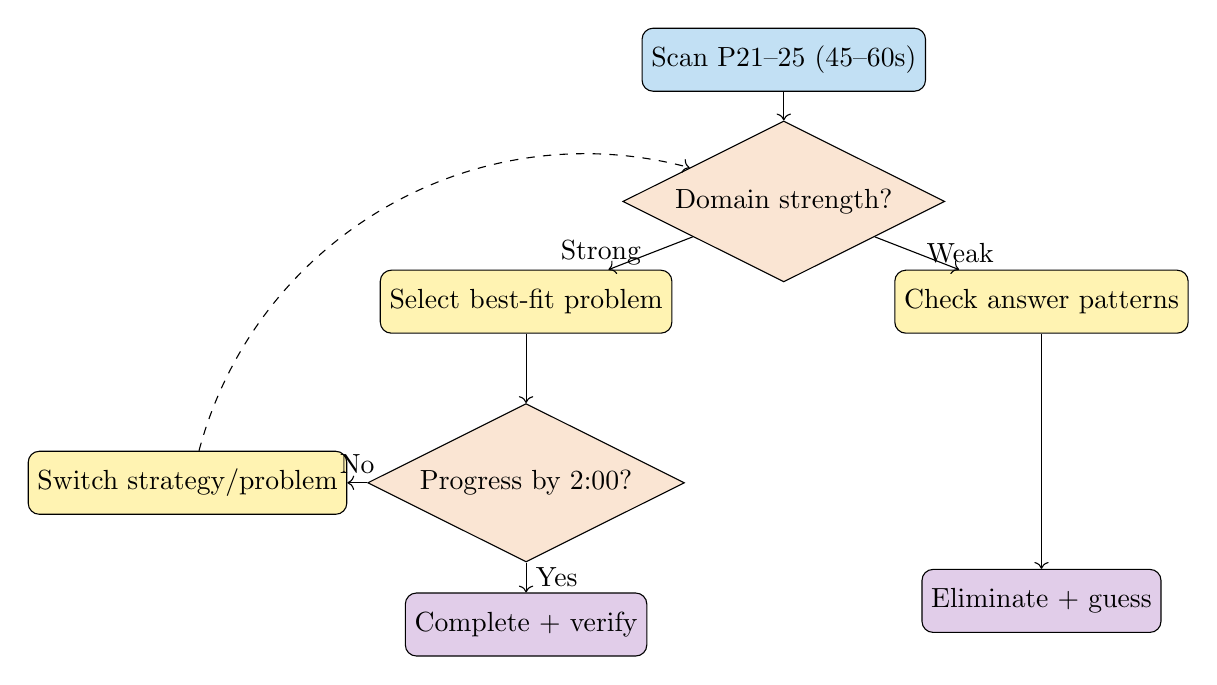
\begin{tikzpicture}[node distance=1.8cm, auto]
    % Define styles
    \tikzstyle{process} = [rectangle, draw, fill=minimalblue!30, rounded corners, minimum width=3cm, minimum height=0.8cm]
    \tikzstyle{decision} = [diamond, draw, fill=targetedorange!20, aspect=2, minimum width=2.5cm]
    \tikzstyle{action} = [rectangle, draw, fill=strategyGold!30, rounded corners, minimum width=2.5cm, minimum height=0.8cm]
    \tikzstyle{verify} = [rectangle, draw, fill=standardpurple!30, rounded corners, minimum width=2.5cm, minimum height=0.8cm]
    
    % Nodes
    \node[process] (start) {Scan P21--25 (45--60s)};
    \node[decision, below of=start] (classify) {Domain strength?};
    \node[action, below left of=classify, xshift=-2cm] (select) {Select best-fit problem};
    \node[action, below right of=classify, xshift=2cm] (leverage) {Check answer patterns};
    \node[decision, below of=select, yshift=-0.5cm] (progress) {Progress by 2:00?};
    \node[action, left of=progress, xshift=-2.5cm] (switch) {Switch strategy/problem};
    \node[verify, below of=progress] (solve) {Complete + verify};
    \node[verify, below of=leverage, yshift=-2cm] (eliminate) {Eliminate + guess};
    
    % Arrows with labels
    \draw[->] (start) -- (classify);
    \draw[->] (classify) -- node[left] {Strong} (select);
    \draw[->] (classify) -- node[right] {Weak} (leverage);
    \draw[->] (select) -- (progress);
    \draw[->] (progress) -- node[above] {No} (switch);
    \draw[->] (progress) -- node[right] {Yes} (solve);
    \draw[->] (leverage) -- (eliminate);
    \draw[->, dashed] (switch) to[bend left=45] (classify);
\end{tikzpicture}
\end{center}

\vspace{1em}
\begin{center}
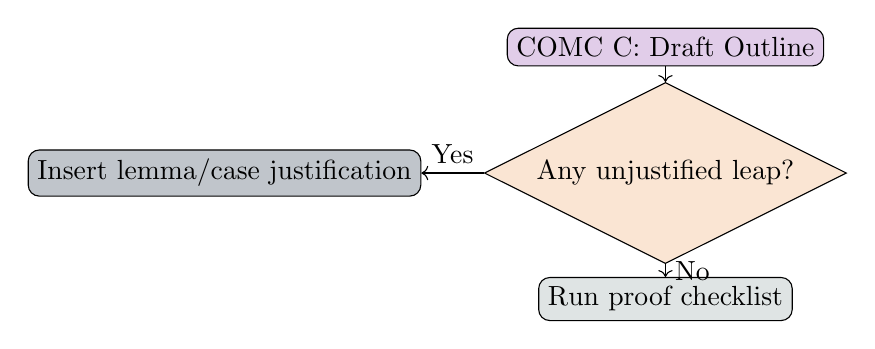
\begin{tikzpicture}[node distance=1.6cm]
    \node[draw, rectangle, fill=standardpurple!30, rounded corners] (cstart) {COMC C: Draft Outline};
    \node[draw, diamond, fill=targetedorange!20, below of=cstart, aspect=2] (gap) {Any unjustified leap?};
    \node[draw, rectangle, fill=formalblack!30, left of=gap, xshift=-4.0cm, rounded corners] (lemma) {Insert lemma/case justification};
    \node[draw, rectangle, fill=completegray!30, below of=gap, rounded corners] (check) {Run proof checklist};
    \draw[->] (cstart) -- (gap);
    \draw[->] (gap) -- node[above] {Yes} (lemma);
    \draw[->] (gap) -- node[right] {No} (check);
\end{tikzpicture}
\end{center}

\newpage

% =============================
% TRAINING PROGRAM
% =============================
\section{Training Program for Late-Band Mastery}

\begin{trainingbox}{Cognitive Load Management System}
    \textit{Three-part framework: externalize, drill weak domains, and trigger simplification.}\\
    \textbf{Simplified Externalization}\\
    \textit{Core principle}: Offload steps to paper to free working memory.\\
    \begin{itemize}[nosep]
        \item \textbf{Algebra}: Write each step; use substitution tables; circle key expressions. \textit{Example}: solving $x^2+2x-3=0$ $\Rightarrow$ let $u=x+1$ so $u^2-4=0$.
        \item \textbf{Geometry}: Sketch diagrams, label givens, mark the goal. \textit{Example}: two chords in a circle—mark intersection and lengths.
        \item \textbf{Number Theory}: Record modular conditions in tables. \textit{Example}: $n\equiv1\pmod 3$, $n\equiv2\pmod 5$.
        \item \textbf{Combinatorics}: List cases systematically. \textit{Example}: ``all different'', ``two same'', ``all same''.
    \end{itemize}
    
    \textbf{Probability \& Combinatorics Drill}\\
    Accuracy often lags here; if these are weak areas:
    \begin{itemize}[nosep]
        \item Dedicate 20--30\% of weekly practice
        \item Emphasize restricted arrangements, complementary counting, expected value
        \item Practice organized casework
        \item Log new techniques in a pattern library
    \end{itemize}
    
    \textbf{Simplification Triggers}\\
    When stuck for more than $90$ seconds, run:
    \begin{enumerate}[nosep]
        \item \textbf{Normalize}: choose convenient origin/scale. \textit{Example}: with $x^2+y^2=1$, set $x=\cos\theta$, $y=\sin\theta$.
        \item \textbf{Specialize}: test $n=2$, equal values, or right angles.
        \item \textbf{Extremize}: probe boundary behavior ($x\to0$, $x\to\infty$).
        \item \textbf{Symmetrize}: impose symmetry; e.g., try $a=b=c$.
    \end{enumerate}
    \end{trainingbox}
    
    \begin{trainingbox}{Metacognitive Monitoring}
    \textbf{Use when}: progress stalls or complexity spikes.\\
    \textbf{The Four Questions}\\
    \begin{enumerate}[nosep]
        \item What am I trying to find? -- Restate the goal.
        \item What haven't I used? -- Check unused constraints.
        \item Is there an easier version? -- Consider simplification.
        \item What would make this trivial? -- Work backwards.
    \end{enumerate}
    \textbf{Progress Indicators}\\
    \begin{itemize}[nosep]
        \item \textbf{Green flags}: expressions simplifying, variables canceling, patterns emerging, constraints satisfied
        \item \textbf{Red flags}: expressions ballooning, new variables needed, algebraic dead ends, constraint violations
    \end{itemize}
\end{trainingbox}
    %\end{multicols}
    

\begin{trainingbox}{Building Your Pattern Recognition Library}
\textbf{Create Problem Signatures}\\
Maintain a notebook organizing problems by their ``signature'' rather than traditional topic categories.

\begin{center}
\begin{tabularx}{\textwidth}{@{}X|X|X|X|X@{}}
\toprule
\textbf{Signature} & \textbf{Primary Approach} & \textbf{Secondary Approach} & \textbf{Example Trigger} & \textbf{Source} \\
\hline
Three variables, symmetric expression & Symmetric polynomials & AM--GM if positive & $a^3 + b^3 + c^3 - 3abc$ & AMC12 2021 P22 \\
\hline 
Recursion with initial values & Compute small cases & Characteristic equation & $a_{n+2} = pa_{n+1} + qa_n$ & COMC 2020 Part C \\
\hline
Circle with multiple chords & Power of a Point & Complex coordinates & Intersecting chords with lengths & AMC12 2019 P23 \\
\hline
Floor/ceiling in equation & Casework on fractional part & Graphical analysis & $\lfloor x \rfloor + \lfloor 2x \rfloor = n$ & AMC12 2022 P21 \\
\hline
Optimization with constraint & Lagrange/substitution & AM--GM or Cauchy--Schwarz & Maximize $xy$ subject to $x^2 + y^2 = 1$ & COMC 2021 Part C \\
\hline
\end{tabularx}
\end{center}

Build 15--20 signatures through focused practice. Review and refine weekly.

\textbf{Track pitfalls}: For each signature, note common wrong turns to avoid repeating mistakes.

\textbf{Example Pattern Library Entry}
\begin{quote}\small\ttfamily
Signature: ``Three variables, symmetric expression''\\
Primary Approach: Symmetric polynomials\\
Secondary Approach: AM-GM if positive\\
Example Trigger: $a^3 + b^3 + c^3 - 3abc$\\
Source: AMC12 2021 P22
\end{quote}

\textbf{Practice Resources (Prioritized for 6--7 weeks):}
\begin{itemize}[nosep]
    \item \textbf{AMC12 Problems}: Focus on 2018--2024 P16--25 (aops.com archives)
    \item \textbf{COMC Problems}: 2019--2024 Part C problems (Canadian Mathematical Society)
    \item \textbf{Additional Practice}: Older AMC12 P21--25 problems for extra ``expansion'' practice
\end{itemize}

\textbf{Problem Selection Guide}
\begin{itemize}[nosep]
    \item 70\% Stretch: AMC12 P18--23 (just beyond current ability)
    \item 20\% Expansion: COMC Part C, harder AMC12 P21--23 (new techniques)
    \item 10\% Impossible: AMC12 P24--25 (creative thinking)
\end{itemize}

\textbf{Topic-Specific Focus (If Needed)}
\begin{itemize}[nosep]
    \item Probability \& Combinatorics: often have lower accuracy rates
    \item Advanced Geometry: complex coordinate geometry and synthetic proofs
    \item Number Theory: modular arithmetic, divisibility, and Diophantine equations
    \item Advanced Algebra: polynomial manipulation, inequalities, and functional equations
\end{itemize}

\emph{Use your problem log to identify patterns in errors---if you consistently struggle with certain topics, dedicate 20--30\% of your practice time to those areas for 1--2 weeks.}

\textbf{Solution Resources}
\begin{itemize}[nosep]
    \item Official MAA solutions for AMC12
    \item AoPS forums for multiple approaches
    \item Canadian Mathematical Society solutions for COMC
    \item \textbf{Pro tip}: After solving, always check 2--3 different solution methods to expand your pattern library
\end{itemize}

\textbf{Community Support (Don't Study in Isolation)}
\begin{itemize}[nosep]
    \item \textbf{AoPS Forums}: Post questions about difficult problems, share solutions
    \item \textbf{Study Groups}: Find a friend or online study partner for weekly problem discussions
    \item \textbf{Math Clubs}: Join your school's math club or online contest math communities
    \item \textbf{Mentorship}: If possible, find an experienced contest math student or teacher for occasional guidance
\end{itemize}

\textbf{Practical Tools and Accountability}
\begin{itemize}[nosep]
    \item \textbf{Digital Tracking}: Use a simple spreadsheet for problem logs and timing (Google Sheets, Excel, or a basic notebook)
    \item \textbf{Timer Tools}: Use phone timer or online timers to track problem-solving time and build pacing awareness
    \item \textbf{Accountability Partner}: Find someone to share weekly progress with
    \item \textbf{Study Environment}: Set up a consistent, distraction-free workspace for practice sessions
    \item \textbf{Reward System}: Set small rewards for reaching weekly goals
\end{itemize}

\textbf{Addressing Content Gaps}
\begin{enumerate}[nosep]
    \item Identify the gap: What specific concept or method is needed?
    \item Quick learning: Use AoPS textbooks, Khan Academy, or YouTube for targeted learning
    \item Practice immediately: Find 3--5 similar AMC12 or COMC problems to solidify understanding
    \item Add to pattern library: Document the new technique with examples
    \item Don't get stuck: If a technique takes too long to learn, skip that problem and return later
\end{enumerate}
\end{trainingbox}

\begin{trainingbox}{Weekly Structure}
\begin{itemize}
    \item \textbf{3 sessions AMC late band} (45--60m): mixed 21--25 practice with triage and closing drills.
    \item \textbf{2 sessions COMC C} (60--75m): one proof write-up, one proof skeleton and check.
    \item \textbf{1 full mock} (75--90m AMC or 150m COMC): simulate pressure; post-mortem with mistake log.
\end{itemize}
\end{trainingbox}

\begin{specializedbox}{Curated Practice Resources}
\textbf{AMC12 P21--25 Training Sets} (in order of priority):
\begin{enumerate}[nosep]
\item Recent AMC12A/B (2020--2024): P21--25 from each exam
\item AIME Problems 1--5: Similar difficulty, different format
\item AoPS Contest Collections: Filter for difficulty 4--5
\item ARML Power Contest: Team problems adaptable for individual practice
\end{enumerate}

\textbf{COMC Part C Preparation}:
\begin{enumerate}[nosep]
\item Past COMC exams (2015--2023): Focus on C1--C2 initially
\item CMO Qualifying Round: Similar proof requirements
\item Putnam A1--A2 problems: Slightly harder but excellent practice
\item IMO Shortlist C1--C3: Combinatorics proof techniques
\end{enumerate}

\textbf{Online Platforms}:
\begin{itemize}[nosep]
\item \textbf{AoPS Alcumus}: Set custom difficulty 4--6
\item \textbf{Brilliant.org}: Advanced problem-solving courses
\item \textbf{CEMC Courseware}: Free Canadian competition prep
\end{itemize}
\end{specializedbox}

\begin{contextbox}{Mistake Analysis Protocol}
Maintain a log categorizing \emph{computational}, \emph{conceptual}, and \emph{strategic} errors. For each error, record prevention: a verification step, a cue to trigger a different conversion, or a time checkpoint rule.
\end{contextbox}

\begin{warningbox}{Common Failure Modes}
\begin{itemize}
    \item Over-solving without leveraging choices (AMC): always attempt bounds/mod/parity first.
    \item Under-justifying (COMC): every non-obvious step needs a reason; state and check conditions of theorems.
    \item Triage drift: sticking beyond time checkpoints; set timers and obey them.
\end{itemize}
\end{warningbox}

% =============================
% CONCLUSION
% =============================
\section{Conclusion}

\begin{successbox}{Key Takeaways}
\begin{enumerate}
    \item \textbf{Access over order}: Pick late-band AMC problems by fit, not index.
    \item \textbf{Engineer the finish}: Aim solutions at answer forms (AMC) or proof skeletons (COMC).
    \item \textbf{Right-size verification}: Standard/Thorough closes for AMC; Complete/Formal elements for COMC.
    \item \textbf{Practice under constraints}: Time checkpoints and proof hygiene are trained skills.
\end{enumerate}
\end{successbox}

\vfill
\begin{center}
\textit{Master late-band strategy, and you turn the hardest points into your competitive edge.}
\end{center}

\newpage
% =============================
% APPENDIX: QUICK REFERENCE CARD
% =============================
\section*{Appendix: Late-Band Quick Reference Card}

\begin{tcolorbox}[colback=strategyGold!5, colframe=strategyGold!75!black, title={\textbf{AMC12 P21--25 Quick Reference}}, fonttitle=\bfseries]
\begin{multicols}{2}
\textbf{Time Checkpoints:}
\begin{itemize}[nosep, leftmargin=*]
\item Initial scan: 45--60s
\item Per problem: 3--4m max
\item Switch trigger: 3:00 no progress
\item Verification: 30--60s
\end{itemize}

\textbf{Strategy Priority:}
\begin{enumerate}[nosep, leftmargin=*]
\item Answer-Choice Leverage (75--90\%)
\item Make It Easier (70--85\%)
\item Penultimate Step (65--80\%)
\item Wishful Thinking (60--75\%)
\item Small Cases (55--70\%)
\end{enumerate}
\end{multicols}

\textbf{Domain-Specific First Moves:}
\begin{itemize}[nosep]
\item \textbf{Algebra}: Check factorability $\to$ Vieta's $\to$ substitution
\item \textbf{Number Theory}: Test mod 2,3,5 $\to$ check small cases $\to$ find pattern
\item \textbf{Combinatorics}: Count small $n$ $\to$ find recursion $\to$ check PIE
\item \textbf{Geometry}: Normalize position $\to$ Power of Point $\to$ coordinates
\end{itemize}
\end{tcolorbox}

\begin{tcolorbox}[colback=standardpurple!5, colframe=standardpurple!75!black, title={\textbf{COMC Part C Quick Reference}}, fonttitle=\bfseries]
\begin{multicols}{2}
\textbf{Time Allocation:}
\begin{itemize}[nosep, leftmargin=*]
\item Part A+B: 60--80m
\item Part C: 70--90m
\item Per C problem: 15--25m
\item Proof outline: 3--5m
\end{itemize}

\textbf{Proof Checklist:}
\begin{enumerate}[nosep, leftmargin=*]
\item State claim precisely
\item Define all variables
\item Justify each step
\item Check all cases
\item Verify boundaries
\item Conclude explicitly
\end{enumerate}
\end{multicols}

\textbf{Partial Credit Maximizers:}
\begin{itemize}[nosep]
\item State approach even if incomplete
\item Show key lemmas/observations
\item Handle base cases in induction
\item Draw clear diagrams with labels
\end{itemize}
\end{tcolorbox}

\begin{tcolorbox}[colback=warningred!5, colframe=warningred!75!black, title={\textbf{Emergency Protocols}}, fonttitle=\bfseries]
\textbf{AMC12 - 10 minutes left:}
\begin{itemize}[nosep]
\item Stop new attempts
\item Verify completed work
\item Use answer elimination on 2--3 accessible unsolved
\item Leave hardest blank (1.5 > 1.2 EV)
\end{itemize}

\textbf{COMC - 20 minutes left:}
\begin{itemize}[nosep]
\item Outline remaining proofs
\item State key observations
\item Show partial work for credit
\item Check arithmetic in completed proofs
\end{itemize}
\end{tcolorbox}

\end{document}

